\begin{table}[ht]
\centering
\begin{tabular}{|c|c|c|c|c|c|c|}
\hline
Descripción & \(V_o\) [V] & \(\Delta V_o\) [V] & \(T\) [ms] & \(\Delta T\) [ms] & \(f\) [kHz] & \(\Delta f\) [kHz] \\ \hline
Oscilando & 9.00 & 1.00 & 0.20 & 0.01 & 5.00 & 0.25 \\ \hline
Saturado & 9.00 & 1.00 & 0.45 & 0.01 & 2.22 & 0.05 \\ \hline
\end{tabular}
\caption{Mediciones de voltaje, periodo y frecuencia del oscilador sin control de amplitud.}
\label{tab:mediciones-voltaje-periodo-oscilador-sin-control}
\end{table}


\begin{table}[ht]
\centering
\begin{tabular}{|c|c|c|c|c|c|c|}
\hline
Descripción & \(R_x\) [k\(\Omega\)] & \(\Delta R_x\) [k\(\Omega\)] & \(RV1\) [k\(\Omega\)] & \(\Delta RV1\) [k\(\Omega\)] & \(X\) & \(\Delta X\) \\ \hline
Oscilando & 4.82 & 0.01 & 10.00 & 0.50 & 0.482 & 0.025 \\ \hline
Saturado & 8.00 & 0.01 & 10.00 & 0.50 & 0.800 & 0.040 \\ \hline
\end{tabular}
\caption{Mediciones del potenciometro en el oscilador sin control de amplitud.}
\label{tab:mediciones-resistencia-oscilador-sin-control}
\end{table}


\begin{ilustracion}[ht]
    \centering
    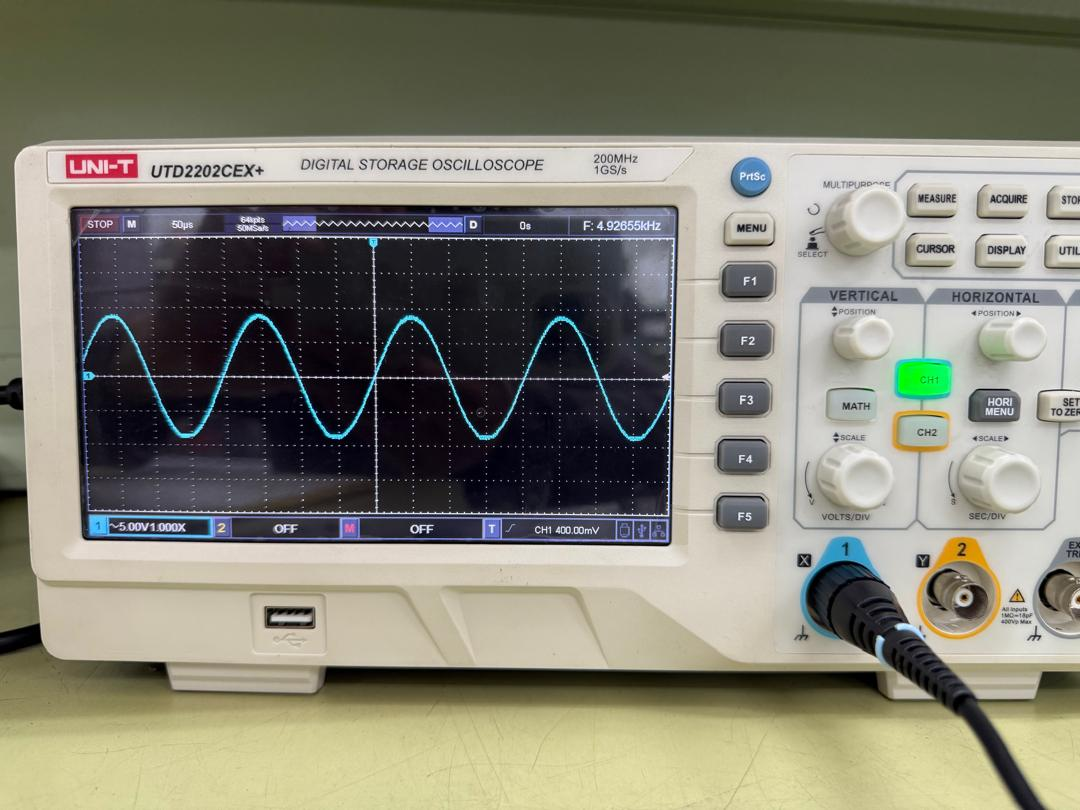
\includegraphics[width=0.6\textwidth]{resultados/oscilador-sin-control-oscilando.jpg}
    \caption{Medición Oscilador sin control de amplitud funcionando.}
    \label{fig:oscilador-sin-control-oscilando}   
\end{ilustracion}

\begin{ilustracion}[ht]
    \centering
    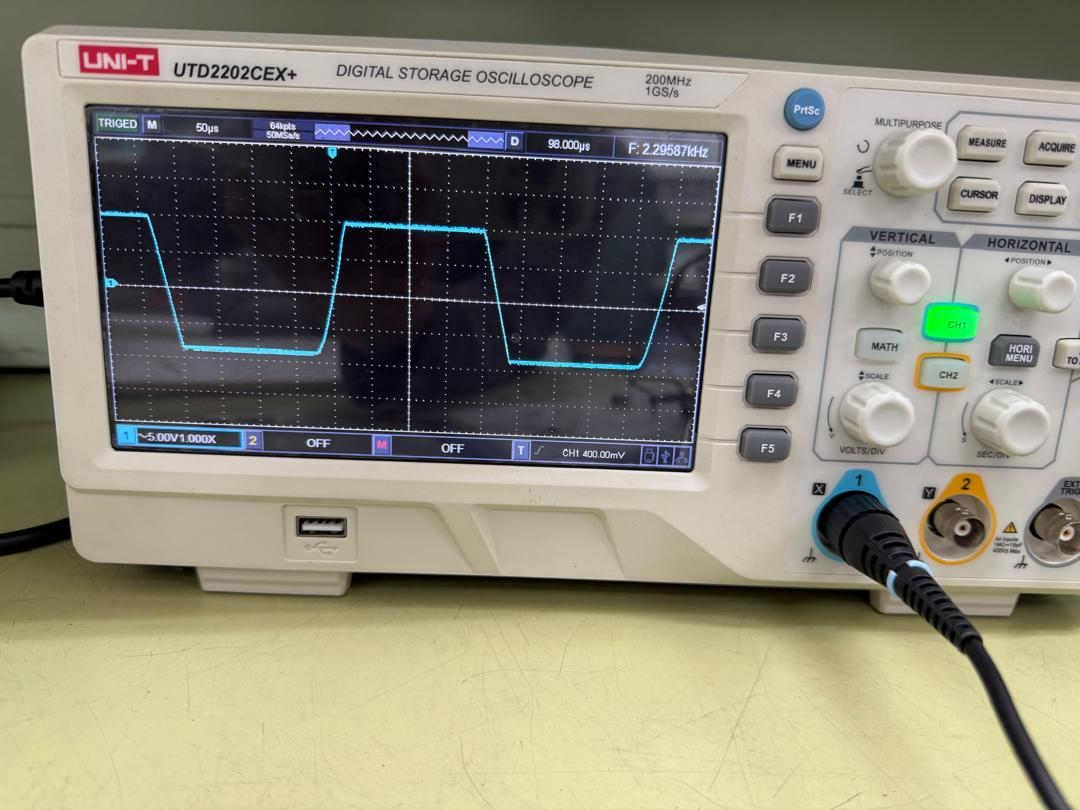
\includegraphics[width=0.6\textwidth]{resultados/oscilador-sin-control-saturado.jpg}
    \caption{Oscilador sin control de amplitud saturado.}
    \label{fig:oscilador-sin-control-saturado}   
\end{ilustracion}

\begin{table}[ht]
\centering
\begin{tabular}{|c|c|c|c|c|c|c|}
\hline
Descripción & \(V_o\) [V] & \(\Delta V_o\) [V] & \(T\) [ms] & \(\Delta T\) [ms] & \(f\) [kHz] & \(\Delta f\) [kHz] \\ \hline
Excursión máxima & 10.00 & 1.00 & 0.22 & 0.01 & 4.55 & 0.21 \\ \hline
Excursión mínima & 0.72 & 0.04 & 0.20 & 0.01 & 5.00 & 0.25 \\ \hline
Saturada & 3.40 & 0.20 & 0.20 & 0.01 & 5.00 & 0.25 \\ \hline
\end{tabular}
\caption{Mediciones de voltaje, periodo y frecuencia del oscilador con control de amplitud.}
\label{tab:mediciones-voltaje-periodo-frecuencia-oscilador-con-control}
\end{table}


\begin{table}[ht]
\centering
\begin{tabular}{|c|c|c|c|c|c|c|}
\hline
Descripción & \(R\) [k\(\Omega\)] & \(\Delta R\) [k\(\Omega\)] & \(RV1\) [k\(\Omega\)] & \(\Delta RV1\) [k\(\Omega\)] & \(X\) & \(\Delta X\) \\ \hline
Excursión máxima & 5.81 & 0.01 & 9.17 & 0.01 & 0.63 & 0.03 \\ \hline
Excursión mínima & 4.84 & 0.01 & 9.17 & 0.01 & 0.52 & 0.03 \\ \hline
Saturada & 6.50 & 0.01 & 9.17 & 0.01 & 0.70 & 0.03 \\ \hline
\end{tabular}
\caption{Mediciones de resistencia del potenciómetro en el oscilador con control de amplitud.}
\label{tab:mediciones-resistencia-oscilador-con-control}
\end{table}

\begin{ilustracion}[ht]
    \centering
    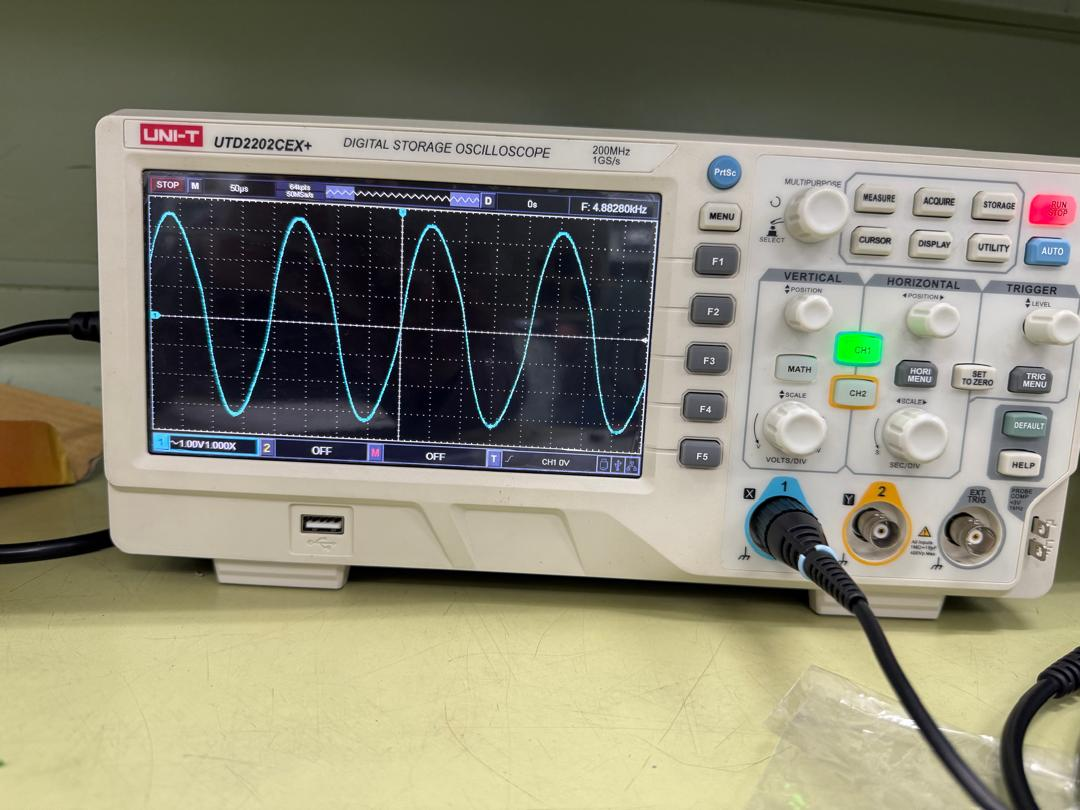
\includegraphics[width=0.6\textwidth]{resultados/oscilador-con-control-max.jpg}
    \caption{Oscilador con control de amplitud en excursión máxima.}
    \label{fig:oscilador-con-control-excursion-maxima}
\end{ilustracion}

\begin{ilustracion}[ht]
    \centering
    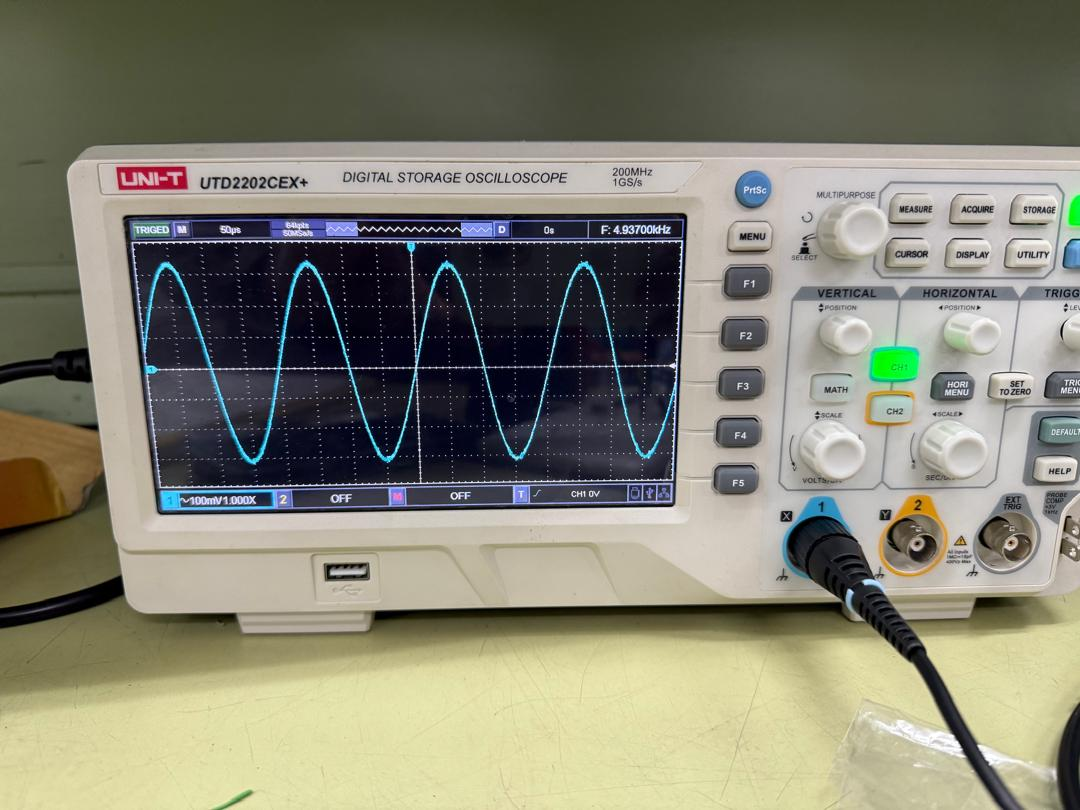
\includegraphics[width=0.6\textwidth]{resultados/oscilador-con-control-min.jpg}
    \caption{Oscilador con control de amplitud en excursión mínima.}
    \label{fig:oscilador-con-control-excursion-minima}
\end{ilustracion}

\begin{ilustracion}[ht]
    \centering
    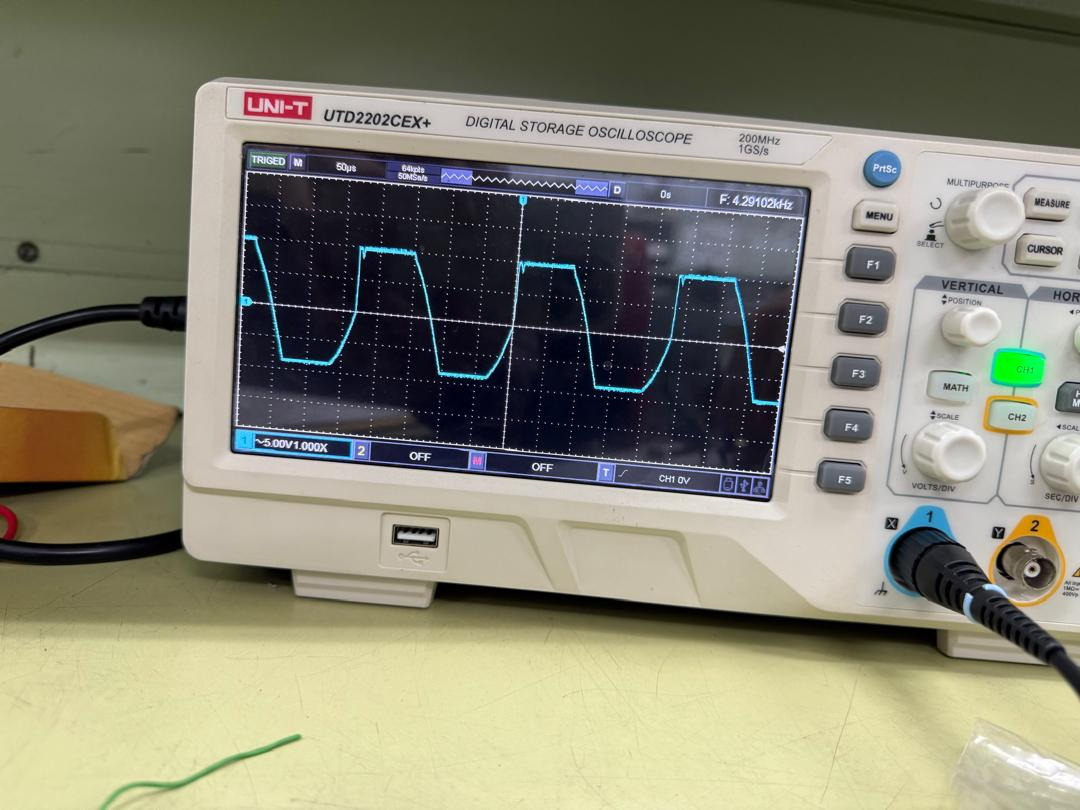
\includegraphics[width=0.6\textwidth]{resultados/oscilador-con-control-saturado.jpg}
    \caption{Oscilador con control de amplitud saturado.}
    \label{fig:oscilador-con-control-saturado}
\end{ilustracion}

\begin{table}[ht]
\centering
\begin{tabular}{|c|c|c|c|c|c|c|}
\hline
Descripción & \(V_o\) [V] & \(\Delta V_o\) [V] & \(V_i\) [V] & \(\Delta V_i\) [V] & \(A\) & \(\Delta A\) \\ \hline
Ganancia oscilador & 5.6 & 0.4 & 1.9 & 0.1 & 2.95 & 0.25 \\ \hline
\end{tabular}
\caption{Mediciones de ganancia del oscilador con control de amplitud.}
\label{tab:mediciones-ganancia-oscilador}
\end{table}

\begin{ilustracion}[ht]
    \centering
    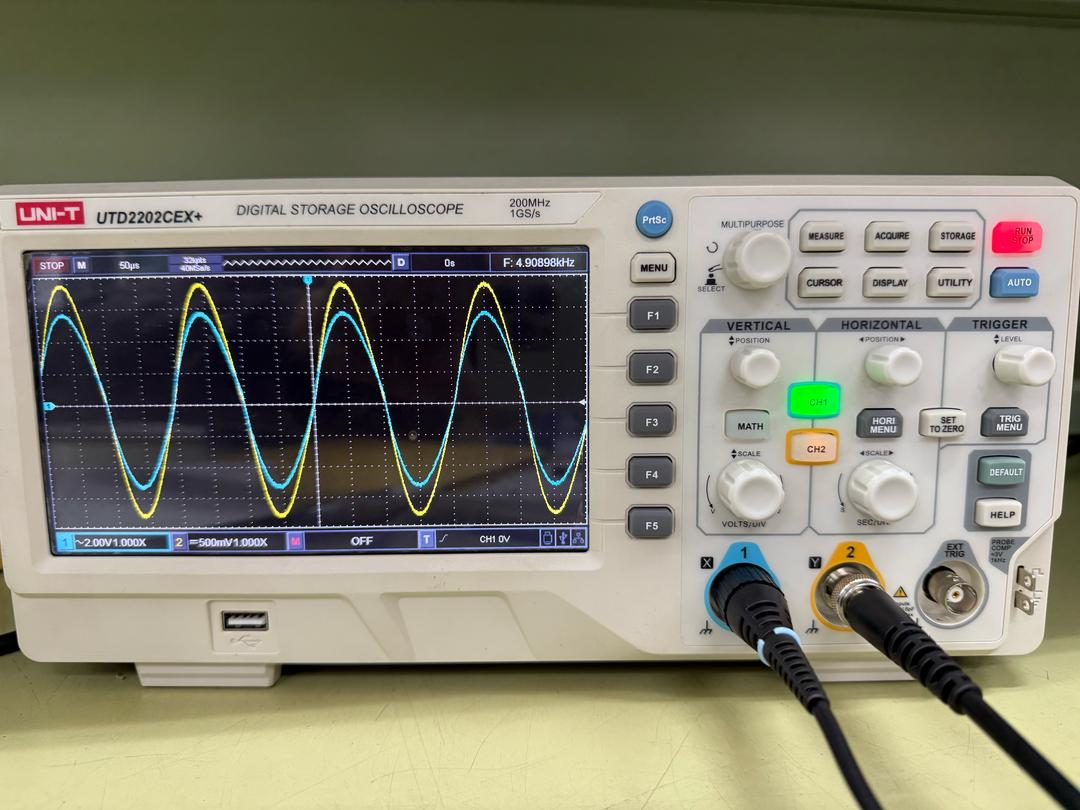
\includegraphics[width=0.6\textwidth]{resultados/oscilador-ganancia.jpg}
    \caption{Medición de la ganancia del oscilador con control de amplitud.}
    \label{fig:oscilador-con-control-ganancia}
\end{ilustracion}
